% Options for packages loaded elsewhere
\PassOptionsToPackage{unicode}{hyperref}
\PassOptionsToPackage{hyphens}{url}
%
\documentclass[
]{article}
\usepackage{amsmath,amssymb}
\usepackage{iftex}
\ifPDFTeX
  \usepackage[T1]{fontenc}
  \usepackage[utf8]{inputenc}
  \usepackage{textcomp} % provide euro and other symbols
\else % if luatex or xetex
  \usepackage{unicode-math} % this also loads fontspec
  \defaultfontfeatures{Scale=MatchLowercase}
  \defaultfontfeatures[\rmfamily]{Ligatures=TeX,Scale=1}
\fi
\usepackage{lmodern}
\ifPDFTeX\else
  % xetex/luatex font selection
\fi
% Use upquote if available, for straight quotes in verbatim environments
\IfFileExists{upquote.sty}{\usepackage{upquote}}{}
\IfFileExists{microtype.sty}{% use microtype if available
  \usepackage[]{microtype}
  \UseMicrotypeSet[protrusion]{basicmath} % disable protrusion for tt fonts
}{}
\makeatletter
\@ifundefined{KOMAClassName}{% if non-KOMA class
  \IfFileExists{parskip.sty}{%
    \usepackage{parskip}
  }{% else
    \setlength{\parindent}{0pt}
    \setlength{\parskip}{6pt plus 2pt minus 1pt}}
}{% if KOMA class
  \KOMAoptions{parskip=half}}
\makeatother
\usepackage{xcolor}
\usepackage[margin=1in]{geometry}
\usepackage{graphicx}
\makeatletter
\def\maxwidth{\ifdim\Gin@nat@width>\linewidth\linewidth\else\Gin@nat@width\fi}
\def\maxheight{\ifdim\Gin@nat@height>\textheight\textheight\else\Gin@nat@height\fi}
\makeatother
% Scale images if necessary, so that they will not overflow the page
% margins by default, and it is still possible to overwrite the defaults
% using explicit options in \includegraphics[width, height, ...]{}
\setkeys{Gin}{width=\maxwidth,height=\maxheight,keepaspectratio}
% Set default figure placement to htbp
\makeatletter
\def\fps@figure{htbp}
\makeatother
\setlength{\emergencystretch}{3em} % prevent overfull lines
\providecommand{\tightlist}{%
  \setlength{\itemsep}{0pt}\setlength{\parskip}{0pt}}
\setcounter{secnumdepth}{-\maxdimen} % remove section numbering
% definitions for citeproc citations
\NewDocumentCommand\citeproctext{}{}
\NewDocumentCommand\citeproc{mm}{%
  \begingroup\def\citeproctext{#2}\cite{#1}\endgroup}
\makeatletter
 % allow citations to break across lines
 \let\@cite@ofmt\@firstofone
 % avoid brackets around text for \cite:
 \def\@biblabel#1{}
 \def\@cite#1#2{{#1\if@tempswa , #2\fi}}
\makeatother
\newlength{\cslhangindent}
\setlength{\cslhangindent}{1.5em}
\newlength{\csllabelwidth}
\setlength{\csllabelwidth}{3em}
\newenvironment{CSLReferences}[2] % #1 hanging-indent, #2 entry-spacing
 {\begin{list}{}{%
  \setlength{\itemindent}{0pt}
  \setlength{\leftmargin}{0pt}
  \setlength{\parsep}{0pt}
  % turn on hanging indent if param 1 is 1
  \ifodd #1
   \setlength{\leftmargin}{\cslhangindent}
   \setlength{\itemindent}{-1\cslhangindent}
  \fi
  % set entry spacing
  \setlength{\itemsep}{#2\baselineskip}}}
 {\end{list}}
\usepackage{calc}
\newcommand{\CSLBlock}[1]{\hfill\break\parbox[t]{\linewidth}{\strut\ignorespaces#1\strut}}
\newcommand{\CSLLeftMargin}[1]{\parbox[t]{\csllabelwidth}{\strut#1\strut}}
\newcommand{\CSLRightInline}[1]{\parbox[t]{\linewidth - \csllabelwidth}{\strut#1\strut}}
\newcommand{\CSLIndent}[1]{\hspace{\cslhangindent}#1}
\usepackage{endfloat}
\usepackage{setspace}\doublespacing
\usepackage{lineno}
\linenumbers
\usepackage{booktabs}
\usepackage{longtable}
\usepackage{array}
\usepackage{multirow}
\usepackage{wrapfig}
\usepackage{float}
\usepackage{colortbl}
\usepackage{pdflscape}
\usepackage{tabu}
\usepackage{threeparttable}
\usepackage{threeparttablex}
\usepackage[normalem]{ulem}
\usepackage{makecell}
\usepackage{xcolor}
\ifLuaTeX
  \usepackage{selnolig}  % disable illegal ligatures
\fi
\usepackage{bookmark}
\IfFileExists{xurl.sty}{\usepackage{xurl}}{} % add URL line breaks if available
\urlstyle{same}
\hypersetup{
  pdftitle={Predicting, habitat suitability, occupancy, and census sizes of a rare plant species using iterative adaptive niche based sampling},
  pdfkeywords={species distribution model, occupancy, census size
estimates,},
  hidelinks,
  pdfcreator={LaTeX via pandoc}}

\title{Predicting, habitat suitability, occupancy, and census sizes of a
rare plant species using iterative adaptive niche based sampling}
\author{Reed Clark Benkendorf\(^1\)\footnote{Author for Correspondence:
  \href{mailto:rbenkendorf@chicagobotanic.org}{\nolinkurl{rbenkendorf@chicagobotanic.org}}},
Jeremie B. Fant\(^1\)\(^,\)\(^2\), Sophie Taddeo\(^3\)\\
\strut ~\(^1\) Chicago Botanic Garden, Glencoe, Illinois 60022, USA\\
\strut ~\(^2\) Plant Biology and Conservation, Northwestern University,
Evanston, Illinois 60208, USA\\
\strut ~\(^3\) Department of Environmental and Ocean Sciences,
University of San Diego, San Diego, California 92110, USA}
\date{}

\begin{document}
\maketitle
\begin{abstract}
\begin{enumerate}
\def\labelenumi{\arabic{enumi})}
\tightlist
\item
\item
\item
\item
\end{enumerate}
\end{abstract}

\section{1 \textbar{} INTRODUCTION}\label{introduction}

The effects of anthropogenic stressors, e.g.~land use and climate
change, have lead to a global extinction crisis with estimates of the
number of plant species facing extinction ranging from 20-40\% (Brummitt
\emph{et al.} (\citeproc{ref-brummitt2015green}{2015}), Pimm \& Joppa
(\citeproc{ref-pimm2015many}{2015}), Nic Lughadha \emph{et al.}
(\citeproc{ref-nic2020extinction}{2020})). Determining which plant
species to focus our conservation efforts (e.g.~active restoration,
preserve creation, \emph{ex situ} collections) on requires an array of
data which seldom exist for decision makers (Heywood
(\citeproc{ref-heywood2017plant}{2017})). These data generally outline
simple biological and ecological parameters of species useful for
detailing there rarity and how it's distribution relates to current and
future anthropogenic stressors. Chief amongst these parameters, are the
geographic extent of occurrence (range), the distribution of suitable
habitat - the occupancy of this habitat as well as the spacing of
occupied patches, and the census size of individual (sub-)populations
(Commission (\citeproc{ref-natural2001iucn}{2001}), Faber-Langendoen
\emph{et al.} (\citeproc{ref-faber2012natureserve}{2012}), \emph{USFWS
species status assessment framework}
(\citeproc{ref-usfws2016ssa}{2016})). While these parameters are
relatively simple, characterizing them can be time consuming, generally
requiring extensive field work and travel to field sites - hence they
oftentimes require proxies or heuristics for estimation in conservation
assessments (Juffe-Bignoli \emph{et al.}
(\citeproc{ref-juffe2016assessing}{2016}), Bland \emph{et al.}
(\citeproc{ref-bland2015cost}{2015}), Pelletier \emph{et al.}
(\citeproc{ref-pelletier2018predicting}{2018})). Environmental niche
models (ENMs or Species Distribution Models SDMs) have made enormous and
respectable headway, respectively, in resolving the former two problems
(extent, and occupancy) (Syfert \emph{et al.}
(\citeproc{ref-syfert2014using}{2014}), Anderson
(\citeproc{ref-anderson2023integrating}{2023}), Kass \emph{et al.}
(\citeproc{ref-kass2021improving}{2021})), however the historic mismatch
between the resolution of variables governing species distributions and
the data available to serve as predictors of environmental conditions
have restricted the interpretation and implementation of these models in
highly heterogeneous environments (Guisan \emph{et al.}
(\citeproc{ref-guisan2013predicting}{2013})). Recent advances in
remote-sensing technologies have allowed for the generation of useful
models in these generally biodiverse systems, further these data offer
promise to model additional population parameters (e.g.~census size,
population extents), however the utility and usage of high resolution
have rarely been ground verified or ostensibly reported upon (Chiffard
\emph{et al.} (\citeproc{ref-chiffard2020anbs}{2020})).

Recently, considerable headway has been made in generating statistically
robust environmental niche models (ENM's) spirited by: recent advances
in collecting high-resolution environmental data, compute power,
digitization of natural history museum records and the acquisition of
citizen science records, and statistical methods especially downsampling
(Markham \emph{et al.} (\citeproc{ref-markham2023review}{2023}), Feldman
\emph{et al.} (\citeproc{ref-feldman2021trends}{2021})).\\
However, ENM's are scarcely ground verified, and even more seldom at
landscape scales (A. Lee-Yaw \emph{et al.}
(\citeproc{ref-a2022species}{2022})). Hence, most of our knowledge about
producing ENM's rely on simulated species and data, especially at
spatial resolutions considered relatively coarse to practitioners.\\
An historic complication with the implementation and interpretation of
ENM's is a mismatch between the spatial resolution of the independent
variables available to model the species fundamental niche and the
factors governing the true distribution of populations - the realized
niche (Carscadden \emph{et al.}
(\citeproc{ref-carscadden2020niche}{2020}), Chauvier \emph{et al.}
(\citeproc{ref-chauvier2022resolution}{2022}), Lembrechts \emph{et al.}
(\citeproc{ref-lembrechts2019incorporating}{2019})). Recent papers have
had mixed results regarding the effects of imprecisely mapped occurrence
data on ENM predictions, with indications that models generated in more
heterogenous environments, and at finer resolutions (e.g.~ca. 3
arc-second (\textasciitilde90m???) relative to 10 arc-minutes
(\textasciitilde14.5 km) at 38*)) suffer minor decreases in model
performance (Graham \emph{et al.}
(\citeproc{ref-graham2008influence}{2008}), Smith \emph{et al.}
(\citeproc{ref-smith2023including}{2023})) with real species, while
increasing error in mapping has drastic effects on model predictions
with virtually simulated species (Gábor \emph{et al.}
(\citeproc{ref-gabor2022positional}{2022})).\\
A further mismatch of resolution is the year in which data on geographic
localities were obtained and current conditions which allow for positive
population growth (Bracken \emph{et al.}
(\citeproc{ref-bracken2022maximizing}{2022})). Historic occurrence data
may now represent conditions which are inhospitable to the maintenance
of populations, or may even represent populations which even then were
simply sinks from more robust populations (Bracken \emph{et al.}
(\citeproc{ref-bracken2022maximizing}{2022})); using these records may
decrease model performance. Collecting data on whether areas are
favorable to continued recruitment of individuals from the soil seed
bank, are perhaps more astute than whether long-lived individuals
persist.

ENM models generally suffer from having few, generally spatially biased,
occurrence records to serve as dependent variables, which generally fail
to characterize the ecological breadth of the species (Stolar \& Nielsen
(\citeproc{ref-stolar2015accounting}{2015}), Feeley \& Silman
(\citeproc{ref-feeley2011keep}{2011})). While many ENM's have
high-performance metrics while tested on small subsets of hold-out data,
they are unlikely to detect many new populations during ground
verification (A. Lee-Yaw \emph{et al.}
(\citeproc{ref-a2022species}{2022})). To increase the number of
presences, and absences in sites which are relatively similar to those
harboring presences, which can be used for training models iterative
adaptive-niche based sampling (ANBS) has become increasingly employed
(Guisan \emph{et al.} (\citeproc{ref-guisan2006using}{2006})). In ANBS
cells predicted to have high probabilities of occurrence, or where
models have higher prediction uncertainty, are preferentially visited,
and after each bout of field visits, a new model is fit incorporating
the original data, plus the recently collected data (Mondain-Monval
\emph{et al.} (\citeproc{ref-mondain2024adaptive}{2024})).\\
Using this process not only allows for the acquisition of a larger
number of presences and absences, but also allows for verifying
geolocated coordinates, that historic points are still extent, reducing
model uncertainty, and for the acquisition of additional data such as
census estimates and life stages (Stockwell \& Peterson
(\citeproc{ref-stockwell2002effects}{2002}), Wisz \emph{et al.}
(\citeproc{ref-wisz2008effects}{2008}), Jansen \emph{et al.}
(\citeproc{ref-jansen2022stop}{2022})). However, few studies have
reported field verified ANBS sampling efforts of plant species (Johnson
\emph{et al.} (\citeproc{ref-johnson2023field}{2023}), Borokini \emph{et
al.} (\citeproc{ref-borokini2023iterative}{2023}), Zimmer \emph{et al.}
(\citeproc{ref-zimmer2023field}{2023})).

An ENM predicts a single variable; the probability of suitable habitat
for the taxon (taddeo2024grimes). Although, in most conservation
applications, the insight desired from an ENM is the species realized
distribution ((\citeproc{ref-cite}{\textbf{cite?}})).\\
The bridge between an ENM and a plant populations presence is related to
the dispersal of propagules and the establishment of the population,
rather than distribution of the fundamental niche alone (Engler \&
Guisan (\citeproc{ref-engler2009migclim}{2009})).\\
Calls - and significant progress, have been made for better integration
of SDM predictions with models of dispersal since the rise in popularity
of ENM's (Guisan \& Thuiller
(\citeproc{ref-guisan2005predicting}{2005}), Franklin
(\citeproc{ref-franklin2010moving}{2010})). Most of this progress
focuses on the goal of `connecting' currently suitable to habitat
predicted to be suitable under climate change scenarios (Engler \&
Guisan (\citeproc{ref-engler2009migclim}{2009}), Bocedi \emph{et al.}
(\citeproc{ref-bocedi2014range}{2014})). Accordingly, ground
verification has not been made for them, nor has as much effort
seemingly been made in attempting to simply improve ground-verification
for rare species\ldots{} To assist practitioners in detecting new
populations, or extending the range of currently known populations, we
propose modelling plant occupancy as a random variable dependent on
distance from sites known to be occupied, the size and shape of the
target site, and it's relation to other suitable habitats.\\
In a simple sense these perspectives link habitat suitability with the
tenets of island biogeography (@). `Distance' may be defined as
euclidean (or Haversine for large distances), or as a least-cost
distance reflecting a generalized surface which conveys the difficulty
for seeds to travel between the nearest occupied sites and the site of
interest (Etherington (\citeproc{ref-etherington2016least}{2016})).\\
Landscape metrics postulated to relate to the occupancy at a site
include the patch metrics Core Area Index, roughly reflecting the
probability of a propagule arriving to a larger patch, and the class
metrics proximity and contagion both of which reflect the aggregation
between occupied sites.

Obtaining reliable estimates of plant population census sizes can be
time intensive process because it requires two major pieces of
information 1) measurements of plant density and 2) population extent.
In lieu of directly determining either the populations boundaries, or
density, observers estimate population sizes, however these estimates
are often unreliable (Reisch \emph{et al.}
(\citeproc{ref-ReischChristoph2018Acom}{2018})). Several promising field
methods for acquiring density measurements have recently been developed
(Rominger \& Meyer (\citeproc{ref-rominger2019application}{2019}),
Krening \emph{et al.} (\citeproc{ref-krening2021sampling}{2021}),
Ermakova \emph{et al.} (\citeproc{ref-ermakova2021densities}{2021}),
Alfaro-Saiz \emph{et al.} (\citeproc{ref-alfaro2019optimal}{2019}),
Schorr (\citeproc{ref-schorr2013using}{2013})) to better estimate
effective population census size (\emph{N}), as well as progress in the
application of genomic methods to estimate effective population sizes
(\emph{N\textsubscript{e}}) (e.g.~linkage disequilibrium) (Waples
(\citeproc{ref-waples2024practical}{2024})). However these methods are
focused on descriptive, rather than predictive processes, where they
focus on estimating the uncertainty in measurements \emph{within} a
population, rather than across the species range. We propose that
estimates of plant density are best generated via methods which allow
for the fitting of statistical models, which can incorporate spatial
covariates and predict estimates and measurements of uncertainty across
gridded surfaces (Oliver \emph{et al.}
(\citeproc{ref-oliver2012population}{2012}), Doser \emph{et al.}
(\citeproc{ref-doser2022spabundance}{2024}), A. Lee-Yaw \emph{et al.}
(\citeproc{ref-a2022species}{2022})).

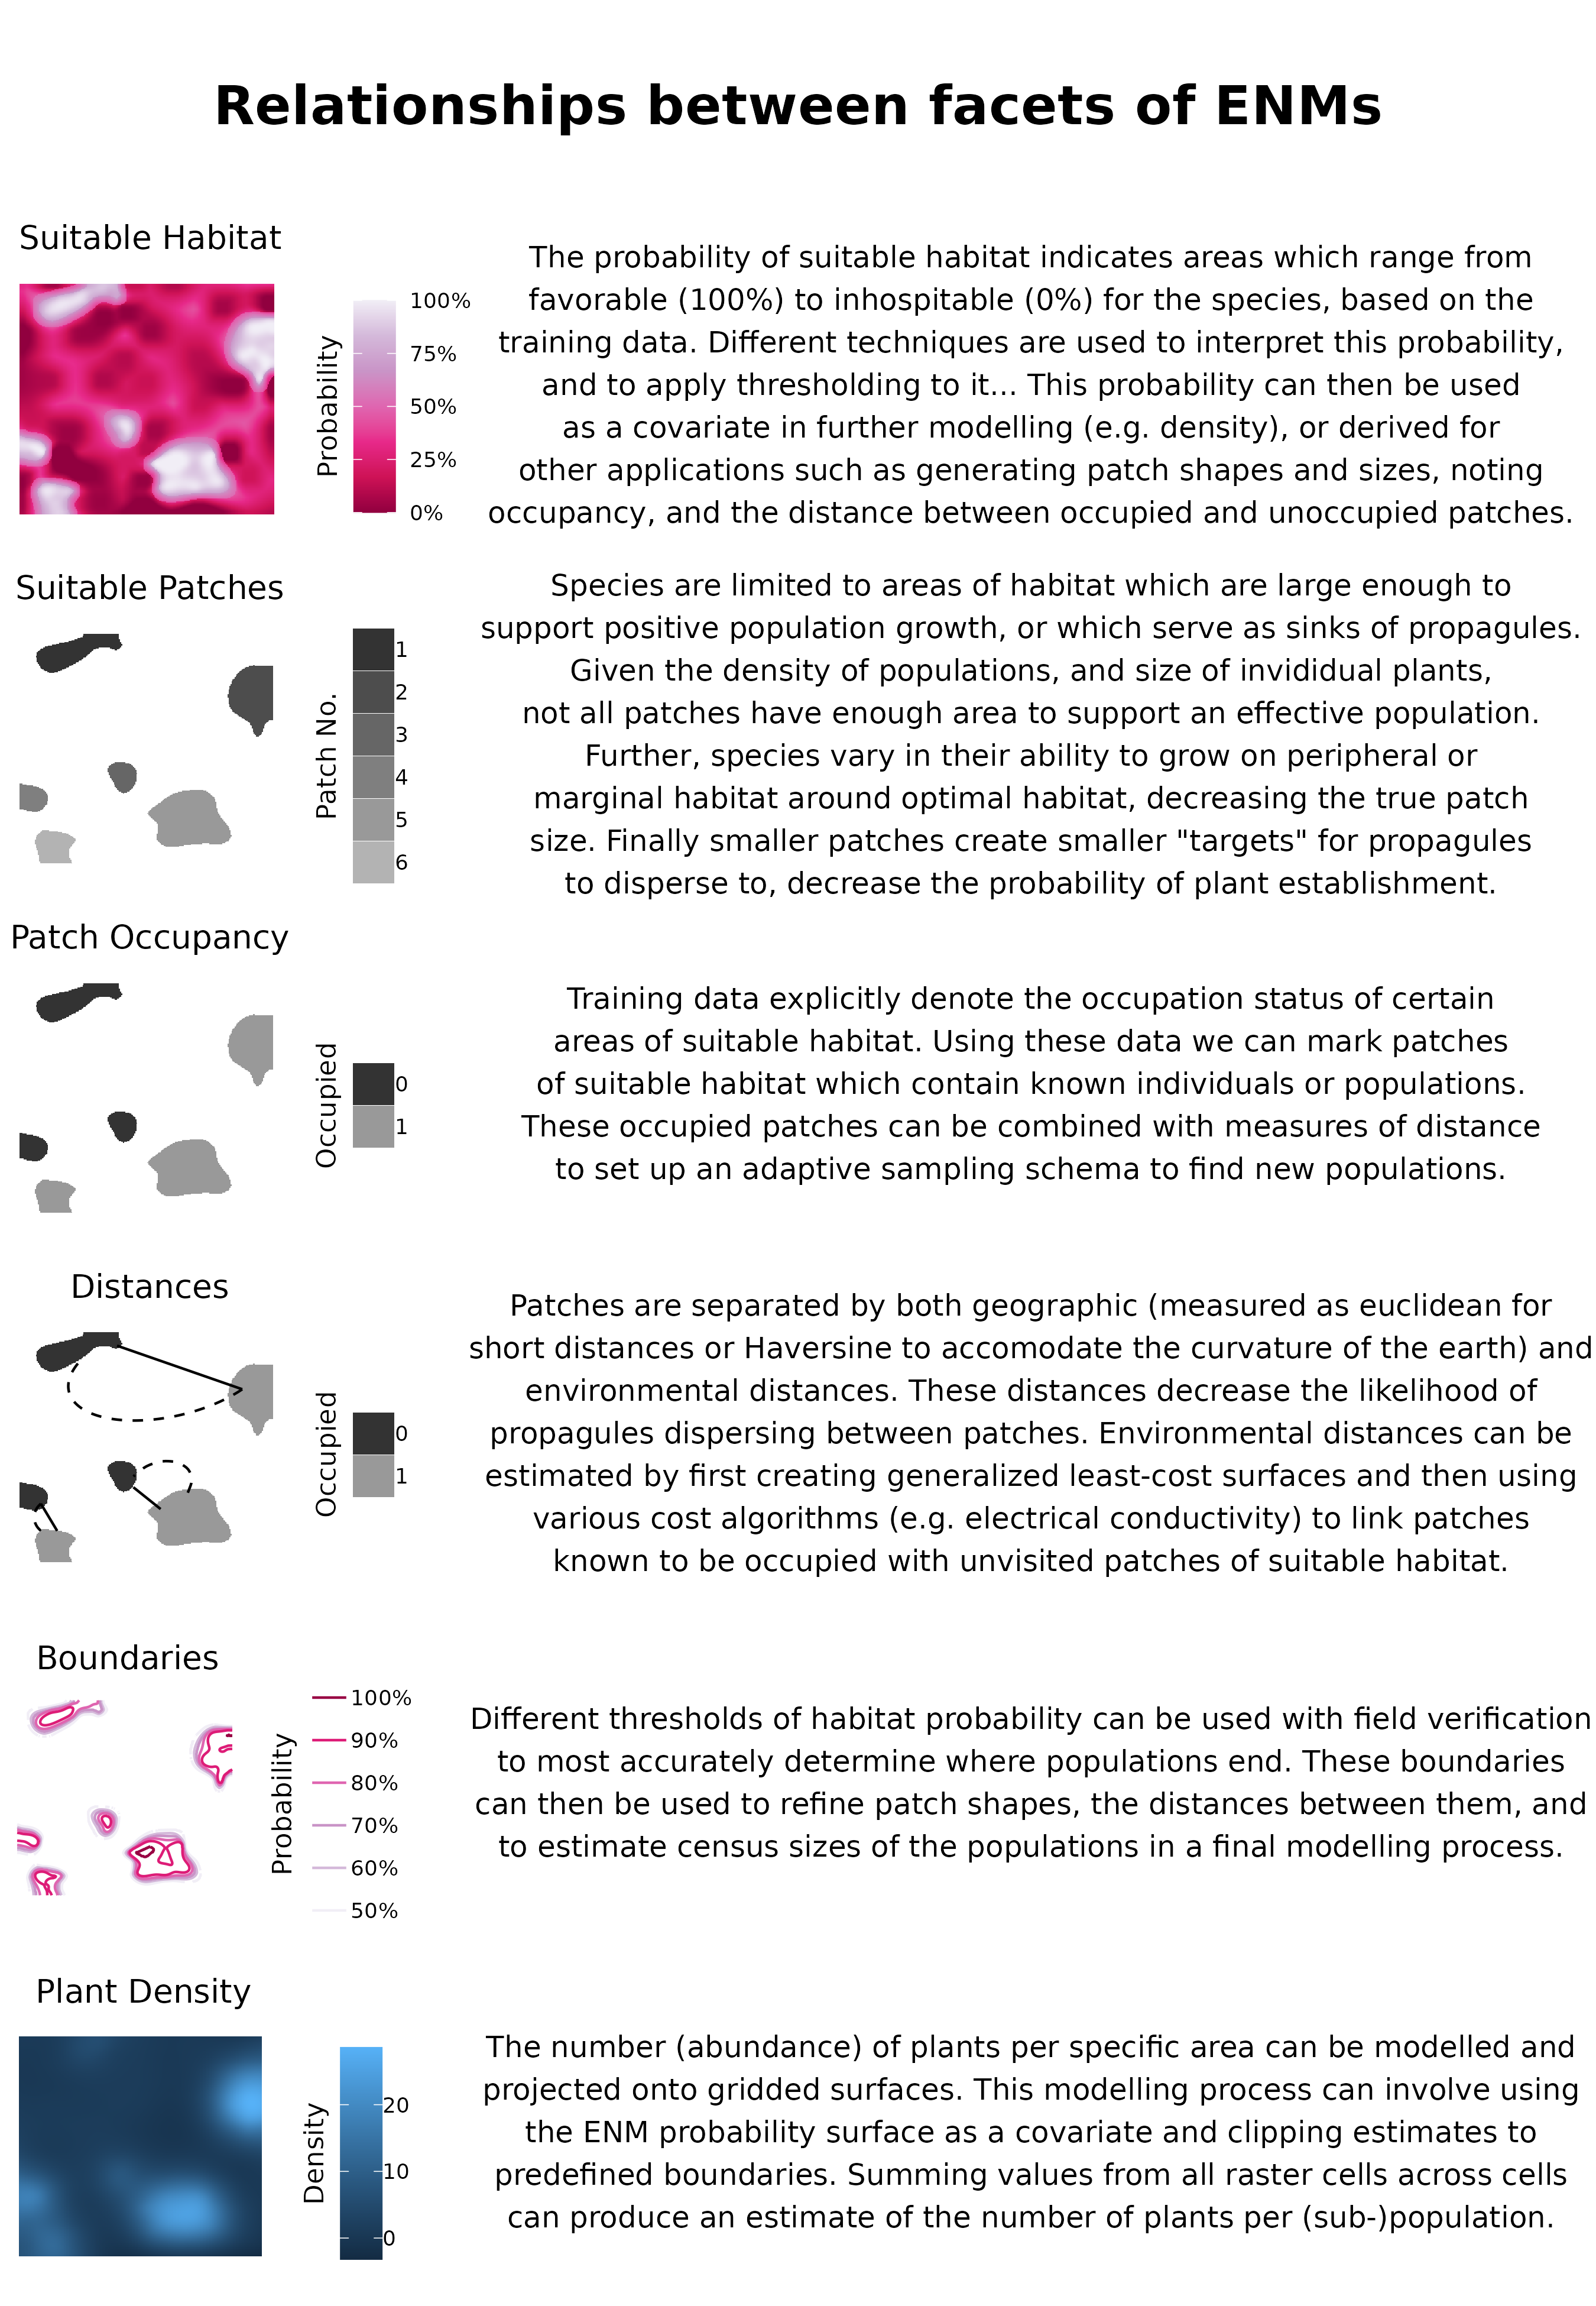
\includegraphics[width=37.5in]{../results/ConceptualFigure}

Mapping the boundaries of a population is another time consuming, albeit
essential task for realistic estimates of population census size.\\
Currently, population boundaries are implicitly delineated by
practitioners walking distances beyond which gene flow between
individuals should be minimal (e.g.~1km) searching for additional
individuals, or via aerial imagery (Elzinga \emph{et al.}
(\citeproc{ref-alma9955306914202441}{1998})).\\
Many rare plant species are small and inconspicuous, and many taxa grow
in small clustered groups in specific habitats, making detection via
either method difficult (Chen \emph{et al.}
(\citeproc{ref-chen2013imperfect}{2013}), Condit \emph{et al.}
(\citeproc{ref-condit2000spatial}{2000})). High resolution spatial data
eventually offer an ability to determine the extent of individual
populations via detection of the edges of suitable habitat.

\section{2 \textbar{} METHODS}\label{methods}

\subsubsection{Study Species \& System}\label{study-species-system}

\emph{Eriogonum coloradense} Small (Polygonaceae) is a synoecious mat
forming perennial herb endemic to the Central Southern Rocky Mountains
in Colorado, U.S.A. It's known geographic range covers XX
km\textsuperscript{2}, with 26 formally described populations, and it is
thought to occur across a range of elevation, slopes, aspects, soil
types and habitats. It's elevation range spans xx - xx m, and the major
habitat types it's known from include: high elevation sagebrush steppe,
sub-alpine grasslands, and alpine slopes. It is considered an S3/G3
species by NatureServe, and a Tier 2 species by State Wildlife Action
Plan by the Colorado Parks and Wildlife Service.

\subsubsection{Data Acqusition}\label{data-acqusition}

Dependent data were gathered from iNaturalist (80 records) and the
Consortium of Southern Rockies herbaria (131 records) ({`Southern rocky
mountain herbaria portal'}, INATURALIST). These data were manually
reviewed and 16 herbarium records which had low geolocation quality, or
which were georeferenced to localities which did not match their
herbarium labels were removed.

Digital Elevation Models at 3arc (type), and 1arc (type), and Digital
Elevation Products at 1/3 arc, and 1m, resolution were acquired from the
United States Geological Survey and clipped to the domain of analysis (a
rectangle buffered 16km (10 mi). beyond any known population). A 3m
resolution digital elevation model, which is not available at a native
resolution from the USGS for this area, was created by bilinear
resampling of the 1m and 10m data. 1m resolution data were only
available for roughly XX\% of the domain (which contained \%\% of known
populations), the remainder of the species domains 3m data was created
by linear resampling of the 10m DEP, a comparison of these results in
the overlapping region are present in appendix xx. These elevation
products were used to create all geomorphology data sets using
whiteboxTools (Wu \& Brown (\citeproc{ref-wu2022whitebox}{2022})).
Vegetation cover data were made by combining the raster data into
continuous covers: Forested, Shrub, and Herbaceous vegetation Tuanmu \&
Jetz (\citeproc{ref-tuanmu2014global}{2014}).

ClimateNA was used to create a data set at 3 arc-second resolution which
then underwent simple bilinear interpolation to generate products at the
finer resolutions (Wang \emph{et al.}
(\citeproc{ref-wang2016locally}{2016})). Gray co-occurrence level
matrices were produced using the glcm r package using 2023 NAIP aerial
imagery, which underwent bilinear resampling to each resolution, using
default setting but with windows of 5 in both directions (Zvoleff
(\citeproc{ref-zvoleff2020glcm}{2020})).

\subsubsection{Ground Verification}\label{ground-verification}

The first round of ground verification was carried out from
June-September 2024. All pre-existing occurrence points were considered
candidates for revisits and all 24 trails leading to them were marked as
SAMPLE UNITS. Each trail was manually mapped, and buffered 45m in each
direction and XXX random points were drawn, thinned to distances
\textgreater{} XXXm, leaving XXX random plots for assessment. XX trails
were visited, allowing for the assessment of XX random points and XX
occurrences. When conducting field work, all presences of \emph{E.
coloradense} were opportunistically noted, and to better describe the
spread of the population points were subjectively placed, with
consdirations of local abudance, ca. 30-50m from the previous one until
traversing out of the population (n = ). Additionally subjectively
placed absences were also collected in areas which seemed favorable, or
were in close proximity, to \emph{E. coloradense} individuals; this
occurred both in field (n = ) and through use of aerial imagery on a
computer afterwards (n = ).

Adaptive Niche-Based Sampling was carried out in July of 2025. To
determine whether adaptive sampling performed better than alternative
sampling regimes (e.g.~stratified, random), and if it could be improved
by occupancy modelling 30 points were selected for each of the
aforementioned sampling schema plus 30 occupancy points.

\subsubsection{Comparision of Different Spatial
Resolutions}\label{comparision-of-different-spatial-resolutions}

Environmental Niche Models were generated at four spatial resolutions, 3
(\textasciitilde72m), 1 (\textasciitilde24m), and 1/3
(\textasciitilde8m) arc-seconds, and 3m.\\
The details of modelling were similar for each resolution.

Records were thinned to the distance of an hypotenuse of a cell to avoid
replicates (Aiello-Lammens \emph{et al.}
(\citeproc{ref-aeillo2015spthin}{2015})). 1.1 times as many Absence, as
presence, records were generated using the background function with
method environmental distance from sdm (Naimi \& Araujo
(\citeproc{ref-naimi2016sdm}{2016})), these records were then manually
reviewed and six records which were deemed in areas which may be
possible presences were removed, after this the records were randomly
sampled to reduce the data set size to XX records.\\
After the first iteration of modelling all additional presences and
absences were thinned via a similar manner and combined with the
original absence records. `Presences' which had greater coordinate
uncertainty than the resolution of modelling were removed.

All random forest models were fit using the ranger package, 95\%
confidence intervals were generated using the infinitesimal jackknife
(Wager \emph{et al.} (\citeproc{ref-wager2014confidence}{2014}), Wright
\& Ziegler (\citeproc{ref-wright2017ranger}{2017})). The generation of
CI's for the 3m data set were not considered feasible and their
prediction was omitted.

\subsubsection{Adaptive and Occupancy Based Field
Sampling}\label{adaptive-and-occupancy-based-field-sampling}

500 stratified points ranging from 1-100\% probability of suitable
habitat were generated using sample (terra). Occupancy scores for each
of these points were then calculated using (whiteboxtools). 200 points
which maximized the spread of values along both dimensions (habitat,
occupancy) were then chosen for ground verification.

\subsubsection{Plant Density}\label{plant-density}

Plant density was modelled using five methods, a generalized linear
model (GLM) with a poisson error distribution and spatial
autocorrelation structures, spAbundance, Random Forest and XgBoost
regression.

\subsubsection{Species Occupancy}\label{species-occupancy}

\subsection{Comparision of Juvenile and Mature Plant
Models}\label{comparision-of-juvenile-and-mature-plant-models}

Using the top performing model resolution () models were refit using
only either juvenile or mature plant presences, the number of mature
presences were limited to the number of juvenile occurrences. Models
were fit at 6 sample sizes (n = 15, 30, 50, 75, 125, 200) 15 times each
using a randomly sampled 60\%-40\% train-test split of data.

\subsection{Simulations of Sample
Size}\label{simulations-of-sample-size}

The effect of sample size on model performance was simulated at 8 sample
sizes (n = 15, 30, 50, 75, 125, 200, 300, 400) each 25 times, using a
randomly sampled 60\%-40\% train-test split of data.

\subsection{Simulations of Coordinate
Errors}\label{simulations-of-coordinate-errors}

The effect of sample size on model performance was simulated at 6 sample
sizes (n = 15, 30, 50, 75, 125, 200), with three proportions of records
in error (0\%, 5\%, 10\%, 20\%), and 3 levels of coordinate uncertainty
(0m, 10m, 100m, 1000m), at each of the 5 resolutions 25 times.

\subsection{3 \textbar{} RESULTS}\label{results}

\subsubsection{Comparision of Different Spatial
Resolutions}\label{comparision-of-different-spatial-resolutions-1}

The area under the receiver operating curve (AUC-ROC) and
precision-recall curve (AUC-PR), the True Skill Statistic, and
Sensitivity and Specificity (Sofaer \emph{et al.}
(\citeproc{ref-sofaer2019area}{2019}), Allouche \emph{et al.}
(\citeproc{ref-allouche2006assessing}{2006})).

\subsubsection{Ground Verification}\label{ground-verification-1}

\subsubsection{Plant Density}\label{plant-density-1}

\subsubsection{Species Occupancy}\label{species-occupancy-1}

\subsection{Comparision of Juvenile and Mature Plant
Models}\label{comparision-of-juvenile-and-mature-plant-models-1}

\subsection{Simulations of Sample
Size}\label{simulations-of-sample-size-1}

\subsection{Simulations of Coordinate
Errors}\label{simulations-of-coordinate-errors-1}

\subsection{4 \textbar{} DISCUSSION}\label{discussion}

\subsection{5 \textbar{} CONCLUSIONS}\label{conclusions}

\subsection{6 \textbar{} ACKNOWLEDGMENTS}\label{acknowledgments}

\subsection*{REFERENCES}\label{references}
\addcontentsline{toc}{subsection}{REFERENCES}

\phantomsection\label{refs}
\begin{CSLReferences}{1}{1}
\bibitem[\citeproctext]{ref-a2022species}
A. Lee-Yaw, J., L. McCune, J., Pironon, S. \& N. Sheth, S. (2022).
Species distribution models rarely predict the biology of real
populations. \emph{Ecography}, \textbf{2022}, e05877.

\bibitem[\citeproctext]{ref-aeillo2015spthin}
Aiello-Lammens, M.E., Boria, R.A., Radosavljevic, A. \& Vilela, B.
(2015).
\href{https://onlinelibrary.wiley.com/doi/10.1111/ecog.01132}{{spThin}:
An {R} package for spatial thinning of species occurrence records for
use in ecological niche models}. \emph{Ecography}, \textbf{38},
541--545.

\bibitem[\citeproctext]{ref-alfaro2019optimal}
Alfaro-Saiz, E., Granda, V., Rodrı́guez, A., Alonso-Redondo, R. \&
Garcı́a-González, M.E. (2019). Optimal census method to estimate
population sizes of species growing on rock walls: The case of mature
primula pedemontana. \emph{Global Ecology and Conservation},
\textbf{17}, e00563.

\bibitem[\citeproctext]{ref-allouche2006assessing}
Allouche, O., Tsoar, A. \& Kadmon, R. (2006). Assessing the accuracy of
species distribution models: Prevalence, kappa and the true skill
statistic (TSS). \emph{Journal of applied ecology}, \textbf{43},
1223--1232.

\bibitem[\citeproctext]{ref-anderson2023integrating}
Anderson, R.P. (2023). Integrating habitat-masked range maps with
quantifications of prevalence to estimate area of occupancy in IUCN
assessments. \emph{Conservation Biology}, \textbf{37}, e14019.

\bibitem[\citeproctext]{ref-bland2015cost}
Bland, L.M., Orme, C.D.L., Bielby, J., Collen, B., Nicholson, E. \&
McCarthy, M.A. (2015). Cost-effective assessment of extinction risk with
limited information. \emph{Journal of Applied Ecology}, \textbf{52},
861--870.

\bibitem[\citeproctext]{ref-bocedi2014range}
Bocedi, G., Palmer, S.C., Pe'er, G., Heikkinen, R.K., Matsinos, Y.G.,
Watts, K. \& Travis, J.M. (2014). Range s hifter: A platform for
modelling spatial eco-evolutionary dynamics and species' responses to
environmental changes. \emph{Methods in Ecology and Evolution},
\textbf{5}, 388--396.

\bibitem[\citeproctext]{ref-borokini2023iterative}
Borokini, I.T., Nussear, K., Petitpierre, B., Dilts, T.E. \& Weisberg,
P.J. (2023). Iterative species distribution modeling results in the
discovery of novel populations of a rare cold desert perennial.
\emph{Endangered Species Research}, \textbf{50}, 47--62.

\bibitem[\citeproctext]{ref-bracken2022maximizing}
Bracken, J.T., Davis, A.Y., O'Donnell, K.M., Barichivich, W.J., Walls,
S.C. \& Jezkova, T. (2022). Maximizing species distribution model
performance when using historical occurrences and variables of varying
persistency. \emph{Ecosphere}, \textbf{13}, e3951.

\bibitem[\citeproctext]{ref-brummitt2015green}
Brummitt, N.A., Bachman, S.P., Griffiths-Lee, J., Lutz, M., Moat, J.F.,
Farjon, A., Donaldson, J.S., Hilton-Taylor, C., Meagher, T.R.,
Albuquerque, S. \& others. (2015). Green plants in the red: A baseline
global assessment for the IUCN sampled red list index for plants.
\emph{PloS one}, \textbf{10}, e0135152.

\bibitem[\citeproctext]{ref-carscadden2020niche}
Carscadden, K.A., Emery, N.C., Arnillas, C.A., Cadotte, M.W., Afkhami,
M.E., Gravel, D., Livingstone, S.W. \& Wiens, J.J. (2020). Niche
breadth: Causes and consequences for ecology, evolution, and
conservation. \emph{The Quarterly Review of Biology}, \textbf{95},
179--214.

\bibitem[\citeproctext]{ref-chauvier2022resolution}
Chauvier, Y., Descombes, P., Guéguen, M., Boulangeat, L., Thuiller, W.
\& Zimmermann, N.E. (2022). Resolution in species distribution models
shapes spatial patterns of plant multifaceted diversity.
\emph{Ecography}, \textbf{2022}, e05973.

\bibitem[\citeproctext]{ref-chen2013imperfect}
Chen, G., Kéry, M., Plattner, M., Ma, K. \& Gardner, B. (2013).
Imperfect detection is the rule rather than the exception in plant
distribution studies. \emph{Journal of Ecology}, \textbf{101}, 183--191.

\bibitem[\citeproctext]{ref-chiffard2020anbs}
Chiffard, J., Marciau, C., Yoccoz, N.G., Mouillot, F., Duchateau, S.,
Nadeau, I., Fontanilles, P. \& Besnard, A. (2020).
\href{https://doi.org/10.1111/2041-210X.13399}{Adaptive niche-based
sampling to improve ability to find rare and elusive species:
Simulations and field tests}. \emph{Methods in Ecology and Evolution},
\textbf{11}, 899--909.

\bibitem[\citeproctext]{ref-natural2001iucn}
Commission, N.Resources.S.S. (2001). \emph{IUCN red list categories and
criteria}. IUCN.

\bibitem[\citeproctext]{ref-condit2000spatial}
Condit, R., Ashton, P.S., Baker, P., Bunyavejchewin, S., Gunatilleke,
S., Gunatilleke, N., Hubbell, S.P., Foster, R.B., Itoh, A., LaFrankie,
J.V. \& others. (2000). Spatial patterns in the distribution of tropical
tree species. \emph{Science}, \textbf{288}, 1414--1418.

\bibitem[\citeproctext]{ref-doser2022spabundance}
Doser, J.W., Finley, A.O., Kéry, M. \& Zipkin, E.F. (2024).
\href{https://doi.org/10.1111/2041-210X.14332}{spAbundance: An r package
for single-species and multi-species spatially explicit abundance
models}. \emph{Methods in Ecology and Evolution}, \textbf{15},
1024--1033.

\bibitem[\citeproctext]{ref-alma9955306914202441}
Elzinga, C.L., Salzer, D.W. \& Willoughby, J.W. (1998). \emph{Measuring
\& monitoring plant populations}. U.S. Dept. of the Interior, Bureau of
Land Management, Denver, Colo.

\bibitem[\citeproctext]{ref-engler2009migclim}
Engler, R. \& Guisan, A. (2009). MigClim: Predicting plant distribution
and dispersal in a changing climate. \emph{Diversity and distributions},
\textbf{15}, 590--601.

\bibitem[\citeproctext]{ref-ermakova2021densities}
Ermakova, A., Trout, K., Terry, M.K., Whiting, C.V., Clubbe, C. \&
Fowler, N. (2021). Densities, plant sizes, and spatial distributions of
six wild populations of lophophora williamsii (cactaceae) in texas, USA.
\emph{Journal of the Botanical Research Institute of Texas},
\textbf{15}, 149--160.

\bibitem[\citeproctext]{ref-etherington2016least}
Etherington, T.R. (2016). Least-cost modelling and landscape ecology:
Concepts, applications, and opportunities. \emph{Current Landscape
Ecology Reports}, \textbf{1}, 40--53.

\bibitem[\citeproctext]{ref-faber2012natureserve}
Faber-Langendoen, D., Nichols, J., Master, L., Snow, K., Tomaino, A.,
Bittman, R., Hammerson, G., Heidel, B., Ramsay, L., Teucher, A. \&
others. (2012). NatureServe conservation status assessments: Methodology
for assigning ranks. \emph{NatureServe, Arlington, VA}.

\bibitem[\citeproctext]{ref-feeley2011keep}
Feeley, K.J. \& Silman, M.R. (2011). Keep collecting: Accurate species
distribution modelling requires more collections than previously
thought. \emph{Diversity and distributions}, \textbf{17}, 1132--1140.

\bibitem[\citeproctext]{ref-feldman2021trends}
Feldman, M.J., Imbeau, L., Marchand, P., Mazerolle, M.J., Darveau, M. \&
Fenton, N.J. (2021). Trends and gaps in the use of citizen science
derived data as input for species distribution models: A quantitative
review. \emph{PloS one}, \textbf{16}, e0234587.

\bibitem[\citeproctext]{ref-franklin2010moving}
Franklin, J. (2010). Moving beyond static species distribution models in
support of conservation biogeography. \emph{Diversity and
Distributions}, \textbf{16}, 321--330.

\bibitem[\citeproctext]{ref-gabor2022positional}
Gábor, L., Jetz, W., Lu, M., Rocchini, D., Cord, A., Malavasi, M.,
Zarzo-Arias, A., Barták, V. \& Moudrỳ, V. (2022). Positional errors in
species distribution modelling are not overcome by the coarser grains of
analysis. \emph{Methods in Ecology and Evolution}, \textbf{13},
2289--2302.

\bibitem[\citeproctext]{ref-graham2008influence}
Graham, C.H., Elith, J., Hijmans, R.J., Guisan, A., Townsend Peterson,
A., Loiselle, B.A. \& Group, N.P.S.D.W. (2008). The influence of spatial
errors in species occurrence data used in distribution models.
\emph{Journal of Applied Ecology}, \textbf{45}, 239--247.

\bibitem[\citeproctext]{ref-guisan2006using}
Guisan, A., Broennimann, O., Engler, R., Vust, M., Yoccoz, N.G.,
Lehmann, A. \& Zimmermann, N.E. (2006). Using niche-based models to
improve the sampling of rare species. \emph{Conservation biology},
\textbf{20}, 501--511.

\bibitem[\citeproctext]{ref-guisan2005predicting}
Guisan, A. \& Thuiller, W. (2005). Predicting species distribution:
Offering more than simple habitat models. \emph{Ecology letters},
\textbf{8}, 993--1009.

\bibitem[\citeproctext]{ref-guisan2013predicting}
Guisan, A., Tingley, R., Baumgartner, J.B., Naujokaitis-Lewis, I.,
Sutcliffe, P.R., Tulloch, A.I., Regan, T.J., Brotons, L.,
McDonald-Madden, E., Mantyka-Pringle, C. \& others. (2013). Predicting
species distributions for conservation decisions. \emph{Ecology
letters}, \textbf{16}, 1424--1435.

\bibitem[\citeproctext]{ref-heywood2017plant}
Heywood, V.H. (2017). Plant conservation in the anthropocene--challenges
and future prospects. \emph{Plant diversity}, \textbf{39}, 314--330.

\bibitem[\citeproctext]{ref-jansen2022stop}
Jansen, J., Woolley, S.N., Dunstan, P.K., Foster, S.D., Hill, N.A.,
Haward, M. \& Johnson, C.R. (2022). Stop ignoring map uncertainty in
biodiversity science and conservation policy. \emph{Nature Ecology \&
Evolution}, \textbf{6}, 828--829.

\bibitem[\citeproctext]{ref-johnson2023field}
Johnson, S., Molano-Flores, B. \& Zaya, D. (2023). Field validation as a
tool for mitigating uncertainty in species distribution modeling for
conservation planning. \emph{Conservation Science and Practice},
\textbf{5}, e12978.

\bibitem[\citeproctext]{ref-juffe2016assessing}
Juffe-Bignoli, D., Brooks, T.M., Butchart, S.H., Jenkins, R.B., Boe, K.,
Hoffmann, M., Angulo, A., Bachman, S., Böhm, M., Brummitt, N. \& others.
(2016). Assessing the cost of global biodiversity and conservation
knowledge. \emph{PLoS One}, \textbf{11}, e0160640.

\bibitem[\citeproctext]{ref-kass2021improving}
Kass, J.M., Meenan, S.I., Tinoco, N., Burneo, S.F. \& Anderson, R.P.
(2021). Improving area of occupancy estimates for parapatric species
using distribution models and support vector machines. \emph{Ecological
Applications}, \textbf{31}, e02228.

\bibitem[\citeproctext]{ref-krening2021sampling}
Krening, P.P., Dawson, C.A., Holsinger, K.W. \& Willoughby, J.W. (2021).
A sampling-based approach to estimating the minimum population size of
the federally threatened colorado hookless cactus (sclerocactus
glaucus). \emph{Natural Areas Journal}, \textbf{41}, 4--10.

\bibitem[\citeproctext]{ref-lembrechts2019incorporating}
Lembrechts, J.J., Nijs, I. \& Lenoir, J. (2019). Incorporating
microclimate into species distribution models. \emph{Ecography},
\textbf{42}, 1267--1279.

\bibitem[\citeproctext]{ref-markham2023review}
Markham, K., Frazier, A.E., Singh, K.K. \& Madden, M. (2023). A review
of methods for scaling remotely sensed data for spatial pattern
analysis. \emph{Landscape Ecology}, \textbf{38}, 619--635.

\bibitem[\citeproctext]{ref-mondain2024adaptive}
Mondain-Monval, T., Pocock, M., Rolph, S., August, T., Wright, E. \&
Jarvis, S. (2024). Adaptive sampling by citizen scientists improves
species distribution model performance: A simulation study.
\emph{Methods in Ecology and Evolution}.

\bibitem[\citeproctext]{ref-naimi2016sdm}
Naimi, B. \& Araujo, M.B. (2016).
\href{https://doi.org/10.1111/ecog.01881}{Sdm: A reproducible and
extensible r platform for species distribution modelling}.
\emph{Ecography}, \textbf{39}, 368--375.

\bibitem[\citeproctext]{ref-nic2020extinction}
Nic Lughadha, E., Bachman, S.P., Leão, T.C., Forest, F., Halley, J.M.,
Moat, J., Acedo, C., Bacon, K.L., Brewer, R.F., Gâteblé, G. \& others.
(2020). Extinction risk and threats to plants and fungi. \emph{Plants,
People, Planet}, \textbf{2}, 389--408.

\bibitem[\citeproctext]{ref-oliver2012population}
Oliver, T.H., Gillings, S., Girardello, M., Rapacciuolo, G., Brereton,
T.M., Siriwardena, G.M., Roy, D.B., Pywell, R. \& Fuller, R.J. (2012).
Population density but not stability can be predicted from species
distribution models. \emph{Journal of Applied Ecology}, \textbf{49},
581--590.

\bibitem[\citeproctext]{ref-pelletier2018predicting}
Pelletier, T.A., Carstens, B.C., Tank, D.C., Sullivan, J. \& Espı́ndola,
A. (2018). Predicting plant conservation priorities on a global scale.
\emph{Proceedings of the National Academy of Sciences}, \textbf{115},
13027--13032.

\bibitem[\citeproctext]{ref-pimm2015many}
Pimm, S.L. \& Joppa, L.N. (2015). How many plant species are there,
where are they, and at what rate are they going extinct? \emph{Annals of
the Missouri Botanical Garden}, \textbf{100}, 170--176.

\bibitem[\citeproctext]{ref-ReischChristoph2018Acom}
Reisch, C., Schmid, C. \& Hartig, F. (2018). A comparison of methods for
estimating plant population size. \emph{Biodiversity and conservation},
\textbf{27}, 2021--2028.

\bibitem[\citeproctext]{ref-rominger2019application}
Rominger, K. \& Meyer, S.E. (2019). Application of UAV-based methodology
for census of an endangered plant species in a fragile habitat.
\emph{Remote Sensing}, \textbf{11}, 719.

\bibitem[\citeproctext]{ref-schorr2013using}
Schorr, R.A. (2013). Using distance sampling to estimate density and
abundance of saussurea weberi hult{é}n (weber's saw-wort). \emph{The
Southwestern Naturalist}, \textbf{58}, 378--383.

\bibitem[\citeproctext]{ref-smith2023including}
Smith, A.B., Murphy, S.J., Henderson, D. \& Erickson, K.D. (2023).
Including imprecisely georeferenced specimens improves accuracy of
species distribution models and estimates of niche breadth. \emph{Global
Ecology and Biogeography}, \textbf{32}, 342--355.

\bibitem[\citeproctext]{ref-sofaer2019area}
Sofaer, H.R., Hoeting, J.A. \& Jarnevich, C.S. (2019). The area under
the precision-recall curve as a performance metric for rare binary
events. \emph{Methods in Ecology and Evolution}, \textbf{10}, 565--577.

\bibitem[\citeproctext]{ref-soro2024}
Southern rocky mountain herbaria portal.

\bibitem[\citeproctext]{ref-stockwell2002effects}
Stockwell, D.R. \& Peterson, A.T. (2002). Effects of sample size on
accuracy of species distribution models. \emph{Ecological modelling},
\textbf{148}, 1--13.

\bibitem[\citeproctext]{ref-stolar2015accounting}
Stolar, J. \& Nielsen, S.E. (2015). Accounting for spatially biased
sampling effort in presence-only species distribution modelling.
\emph{Diversity and Distributions}, \textbf{21}, 595--608.

\bibitem[\citeproctext]{ref-syfert2014using}
Syfert, M.M., Joppa, L., Smith, M.J., Coomes, D.A., Bachman, S.P. \&
Brummitt, N.A. (2014). Using species distribution models to inform IUCN
red list assessments. \emph{Biological Conservation}, \textbf{177},
174--184.

\bibitem[\citeproctext]{ref-tuanmu2014global}
Tuanmu, M.-N. \& Jetz, W. (2014). A global 1-km consensus land-cover
product for biodiversity and ecosystem modelling. \emph{Global Ecology
and Biogeography}, \textbf{23}, 1031--1045.

\bibitem[\citeproctext]{ref-usfws2016ssa}
\emph{USFWS species status assessment framework: An integrated
analytical framework for conservation 3.4}. (2016). U.S. Fish; Wildlife
Service, 5275 VA-7, Falls Church, VA 22041.

\bibitem[\citeproctext]{ref-wager2014confidence}
Wager, S., Hastie, T. \& Efron, B. (2014). Confidence intervals for
random forests: The jackknife and the infinitesimal jackknife. \emph{The
journal of machine learning research}, \textbf{15}, 1625--1651.

\bibitem[\citeproctext]{ref-wang2016locally}
Wang, T., Hamann, A., Spittlehouse, D. \& Carroll, C. (2016). Locally
downscaled and spatially customizable climate data for historical and
future periods for north america. \emph{PloS one}, \textbf{11},
e0156720.

\bibitem[\citeproctext]{ref-waples2024practical}
Waples, R.S. (2024). Practical application of the linkage disequilibrium
method for estimating contemporary effective population size: A review.
\emph{Molecular Ecology Resources}, \textbf{24}, e13879.

\bibitem[\citeproctext]{ref-wisz2008effects}
Wisz, M.S., Hijmans, R., Li, J., Peterson, A.T., Graham, C., Guisan, A.
\& Group, N.P.S.D.W. (2008). Effects of sample size on the performance
of species distribution models. \emph{Diversity and distributions},
\textbf{14}, 763--773.

\bibitem[\citeproctext]{ref-wright2017ranger}
Wright, M.N. \& Ziegler, A. (2017).
\href{https://doi.org/10.18637/jss.v077.i01}{{ranger}: A fast
implementation of random forests for high dimensional data in {C++} and
{R}}. \emph{Journal of Statistical Software}, \textbf{77}, 1--17.

\bibitem[\citeproctext]{ref-wu2022whitebox}
Wu, Q. \& Brown, A. (2022).
\emph{\href{https://CRAN.R-project.org/package=whitebox}{'Whitebox':
'WhiteboxTools' r frontend}}.

\bibitem[\citeproctext]{ref-zimmer2023field}
Zimmer, S.N., Holsinger, K.W. \& Dawson, C.A. (2023). A field-validated
ensemble species distribution model of eriogonum pelinophilum, an
endangered subshrub in colorado, USA. \emph{Ecology and Evolution},
\textbf{13}, e10816.

\bibitem[\citeproctext]{ref-zvoleff2020glcm}
Zvoleff, A. (2020).
\emph{\href{https://CRAN.R-project.org/package=glcm}{Glcm: Calculate
textures from grey-level co-occurrence matrices (GLCMs)}}.

\end{CSLReferences}

\end{document}
